\section{La méthodologie}
Une des manières la plus simple pour savoir si la méthodologie choisie correspondait bien aux résultats attendus et était bien adaptée est d'analyser les chiffres et les résultats que nous avons obtenus.

La méthode agile \Scrum{} que nous avons choisie nous a permis de bien répartir le travail en fonction de la disponibilité de chacun et de ses compétences techniques. En effet avec une moyenne de 10 user story par sprint sur un total de 54, la durée des sprints (2 semaines) était bien adpatée à notre cycle de développement. Nous avons réalisé 6 sprints avec 2 releases. Cette volonté de découper le travail par tranche de deux semaines était bénéfique dans le sens ou nous avons pu nous adapter aux attentes et aux évolutions des besoins du client. Nous reviendrons sur l'organisation plus bas avec le burnup chart.

Par ailleurs, la couverture des tests qui est aux alentours de 90\% sur la fin du projet nous a permis d'éviter un grand nombre de bugs ainsi que d'en trouver certains qui n'auraient pas forcément été détectés si il n'y avait pas eu de tests. Cependant les bugs par rapport à l'interface (clic sur un bouton qui provoque un plantage de l'application) n'ont pas pu être testé et nous avons du procéder à des tests manuels.

Enfin l'utilisation de GitHub en étroite collaboration avec la méthode agile \Scrum{} a permis de pouvoir travailler depuis chez soit ce qui était indispensable dans ce contexte (nous ne pouvions programmer des mêlées tous les jours à cause des cours, etc). Le nombre de pull requests (95), issues (145), branches (91) et commits (1200) en est une preuve ainsi que la preuve de toute la communication que nous avons mis en place pour gérer ce projet.

\begin{figure}
	\centering
	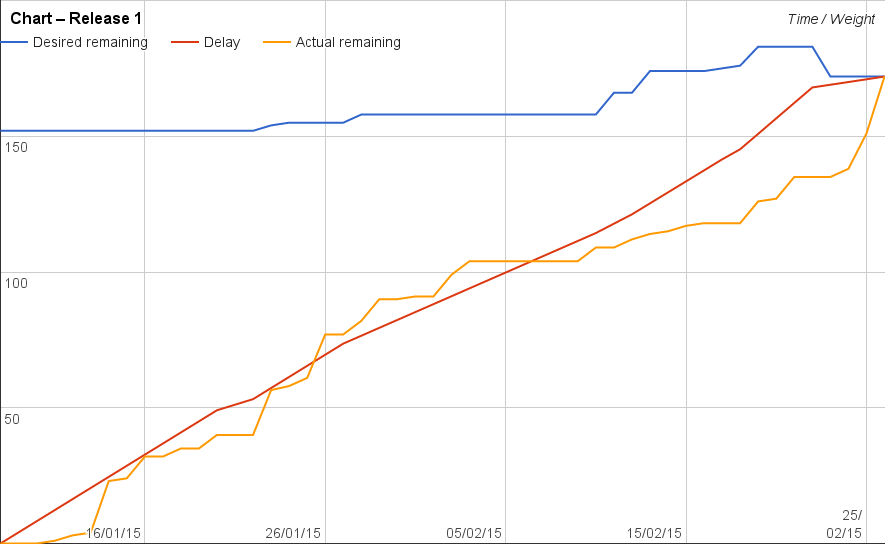
\includegraphics[width=0.9\linewidth]{screens/release1-chart.png}
	\caption{Burn Up chart de la première release}
	\label{fig:burnupchart-release1}
\end{figure}

Dans l’ensemble la courbe suit bien la courbe théorique malgré une tendance en dessous du délai attendu. La coupure du milieu correspond à la semaine de vacances ou nous avons effectué une pause, sur la fin nous avons eu un retard à combler à cause de l’augmentation des stories liée aux bugs. Nous avons du transferérer quelques unes de ces dernières à la release d’après.